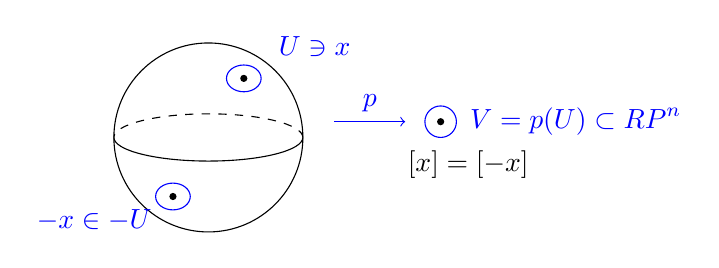
\begin{tikzpicture}
\draw (0,0) circle (1.2);
\draw (-1.2,0) arc (180:360:1.2 and 0.3);
\draw[dashed] (1.2,0) arc (0:180:1.2 and 0.3);
\draw[blue] (0.45,0.75) ellipse (0.22 and 0.17);
\fill (0.45,0.75) circle (1.3pt);
\node[blue] at (1.35,1.15) {$U\ni x$};
\draw[blue] (-0.45,-0.75) ellipse (0.22 and 0.17);
\fill (-0.45,-0.75) circle (1.3pt);
\node[blue] at (-1.45,-1.05) {$-x\in -U$};
\draw[->, blue] (1.6,0.2) -- node[above] {$p$} (2.5,0.2);
\draw[blue] (2.95,0.2) circle (0.2);
\fill (2.95,0.2) circle (1.3pt);
\node[blue, right] at (3.2,0.2) {$V=p(U)\subset\mathbb{RP}^n$};
\node at (3.3,-0.35) {$[x]=[-x]$};
\end{tikzpicture}
